%%
%% CIKM 2026 Applied Research Track (single-blind review).
%% 7 pages including appendix + unlimited pages for GenAI Disclosure & references.
%% ACM Primary Article Template (sigconf, 2-column).
%% See: https://cikm2026.diag.uniroma1.it/applied-research-papers/
%%
\documentclass[sigconf,review]{acmart}
\usepackage{enumitem}
\usepackage{multirow}
\usepackage{pifont}
\usepackage{placeins}
\newcommand{\cmark}{\ding{51}}
\newcommand{\xmark}{\ding{55}}

\setcopyright{acmlicensed}
\copyrightyear{2026}
\acmYear{2026}
\acmDOI{XXXXXXX.XXXXXXX}

\acmConference[CIKM '26]{The 35th ACM International Conference on Information and Knowledge Management}{November 9--11, 2026}{Rome, Italy}
\acmISBN{978-1-4503-XXXX-X/2026/11}

\begin{document}

\title{KAC: KPI-Aware Multimodal Anomaly Detection for High-Dimensional 5G and Open RAN KPI Streams
% KAC: KPI-Aware Multimodal Anomaly Detection for Telecom Observability
}

%% Applied Research Track is SINGLE-BLIND: include real names and affiliations.
\author{Chiman Salavati}
\authornote{Corresponding author.}
\affiliation{%
  \institution{University of Connecticut}
  \city{Storrs}
  \state{CT}
  \country{USA}}
\email{chiman.salavati@uconn.edu}

\author{Liang Wu}
\affiliation{%
  \institution{Nokia}
  \city{Sunnyvale}
  \state{California}
  \country{USA}}
\email{liang.wu@nokia.com}

\author{Kelly Wan}
\affiliation{%
  \institution{Nokia}
  \city{Sunnyvale}
  \state{California}
  \country{USA}}

\author{Mayank Darbari}
\affiliation{%
  \institution{Nokia}
  \city{Sunnyvale}
  \state{California}
  \country{USA}}

\author{Liangjie Hong}
\affiliation{%
  \institution{Nokia}
  \city{Sunnyvale}
  \state{California}
  \country{USA}}

\renewcommand{\shortauthors}{Salavati et al.}

\begin{abstract}
Reliable anomaly detection has become a bottleneck for modern telecom operations, where 5G, Open RAN, and emerging self-optimizing 6G systems must support latency-sensitive applications while tracking hundreds of heterogeneous radio, platform, and packet-level KPIs.
Existing detectors often degrade when moved from offline benchmarks toward production settings, where out-of-distribution operating regimes, severe class imbalance, and high false-alarm costs make purely numerical scores difficult to sustain.
The goal of this work is to make telecom anomaly detection robust to the rapid growth of Open RAN dimensionality while preserving the domain knowledge operators use to decide whether a KPI deviation is actionable.
We present KAC (KPI-Aware Contrastive), a deployment-oriented framework that turns compact operator-style summaries into a learnable feedback signal over full-KPI temporal evidence.
KAC does not ask a language model to make the anomaly decision; instead, it learns which pieces of operational context matter for each KPI, aligns them with the corresponding temporal evidence, and emphasizes signals whose forecasts are reliable.
This gives the detector broad numerical coverage like modern time-series models, while retaining the sparse KPI-specific reasoning that makes operator feedback sustainable after deployment.
Across public 5G telemetry, enterprise-scale Open RAN data, and an industrial 5G packet-trace benchmark produced by Nokia's active cloud-deployed pipeline, KAC outperforms up to 14 trained baselines and three zero-shot frontier LLM baselines.
We release the KAC implementation, benchmark-processing code, and reproducibility artifacts to support deployment-oriented evaluation by telecom operators and benchmark designers.
\end{abstract}

\begin{CCSXML}
<ccs2012>
 <concept>
  <concept_id>10010147.10010257</concept_id>
  <concept_desc>Computing methodologies~Machine learning</concept_desc>
  <concept_significance>500</concept_significance>
 </concept>
</ccs2012>
\end{CCSXML}
\ccsdesc[500]{Computing methodologies~Machine learning}

\keywords{time series, anomaly detection, telecommunications, multimodal learning, contrastive learning, foundation models, deployed systems}

\maketitle

\begin{figure}[!t]
  \centering
  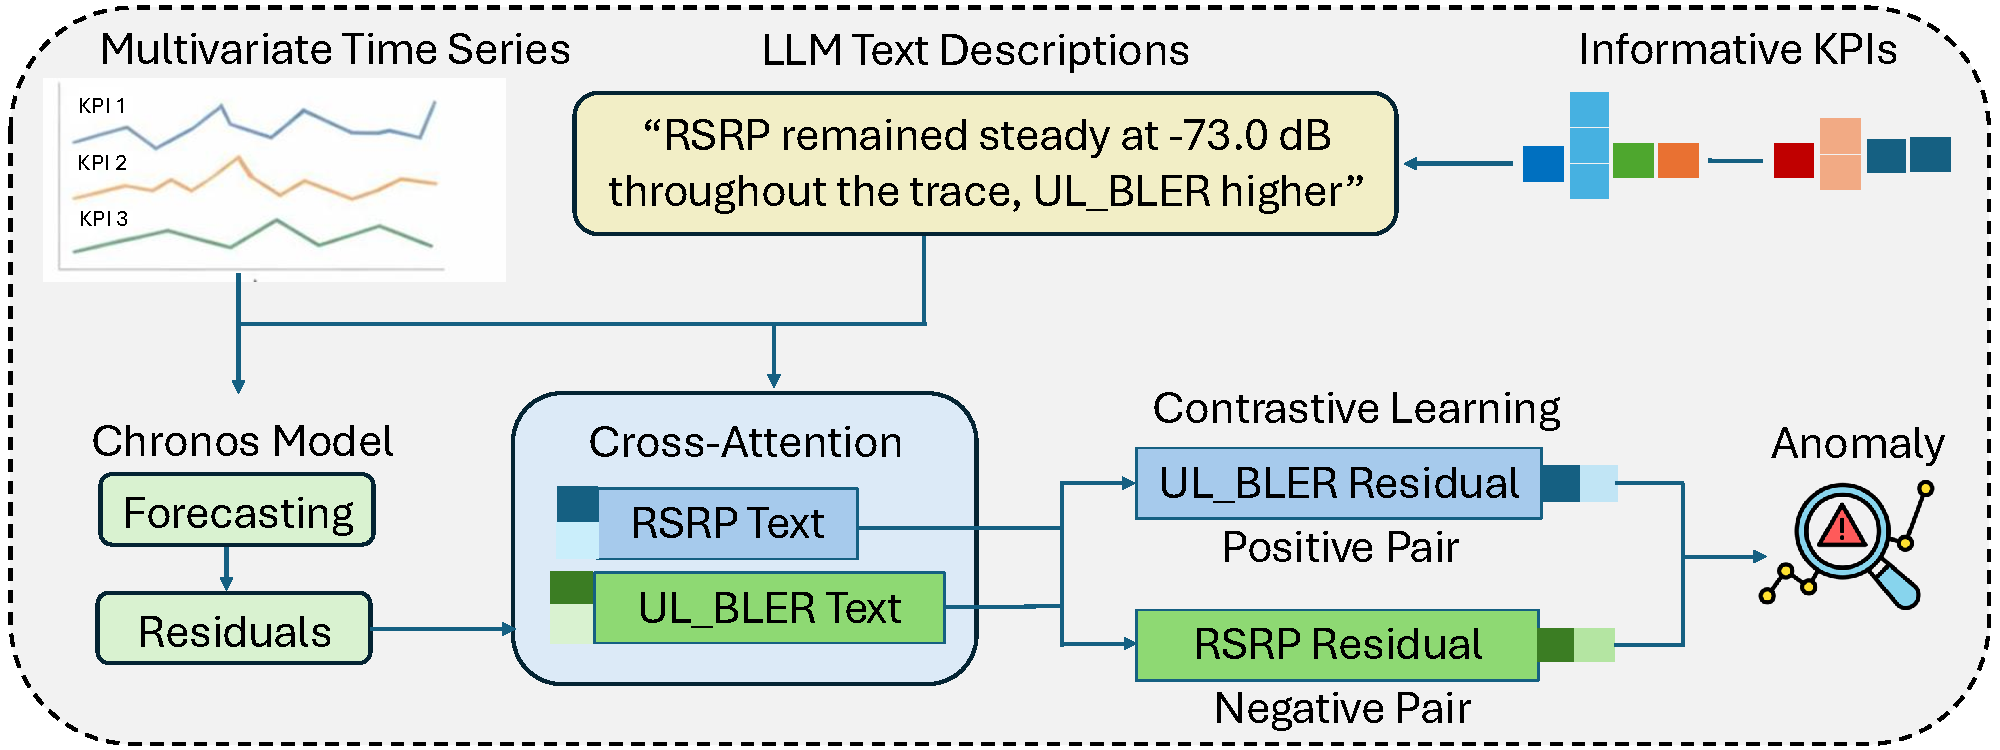
\includegraphics[width=\linewidth]{figures/fig2.pdf}
  \caption{Overview of the proposed KAC pipeline for multimodal telecom anomaly detection.}
  \label{fig:overview}
\end{figure}

\section{Introduction}

Telecom networks are increasingly monitored through observability pipelines that collect heterogeneous KPI time series from 5G and Open RAN deployments.
These measurements feed AIOps workflows for alerting, incident management, and failure diagnosis.
Recent work identifies alert and incident management as a central failure-management task, while dynamic alert-suppression studies show that noisy alert streams remain a practical operational problem~\cite{yu2024alertsurvey,bhukar2024dynamic,zhang2024aiopsllm}.
The challenge is especially acute in Open RAN, where disaggregated and virtualized components increase operational complexity and anomaly detectors must process fine-grained RAN and platform metrics jointly~\cite{sun2024spotlight}.
TelecomTS further shows that 5G observability data are heterogeneous, scale-sensitive, and useful beyond forecasting, supporting anomaly detection, root-cause analysis, and multimodal reasoning~\cite{feng2025telecomts}.
These observations motivate the applied problem studied in this paper: \emph{how can we produce reliable anomaly scores from noisy, high-dimensional telecom KPI windows under false-alarm constraints?}

Multivariate time-series anomaly detection (MTSAD) has been studied extensively~\cite{schmidl2022evaluation,darban2024deep}.
Classical deep approaches such as OmniAnomaly~\cite{su2019omnianomaly}, USAD~\cite{audibert2020usad}, TranAD~\cite{tuli2022tranad}, Anomaly Transformer~\cite{xu2022anomaly}, GDN~\cite{deng2021gdn}, and MTAD-GAT~\cite{zhao2020mtadgat} learn strong numerical representations of normal temporal behavior and inter-variable structure.
However, these models represent variables as numerical channels, graph nodes, or attention patterns rather than explicit KPI identities or operational context.
This limitation matters in telecom observability, where de-anonymized KPI names and absolute scales are operationally meaningful: the same numerical deviation can be benign or suspicious depending on which KPI moved and under what operating regime~\cite{feng2025telecomts}.

Time-series foundation models provide a complementary source of pretrained temporal knowledge.
Chronos formulates forecasting as sequence modeling over quantized time-series values~\cite{ansari2024chronos}, and Chronos-2 extends this line to univariate, multivariate, and covariate-informed zero-shot forecasting~\cite{ansari2025chronos2}.
Other TSFMs such as MOMENT~\cite{goswami2024moment}, Moirai~\cite{woo2024moirai}, and TimesFM~\cite{das2024timesfm} similarly show that large pretrained models can transfer across diverse time-series tasks.
A natural anomaly-detection strategy is therefore to use forecast errors or frozen TSFM embeddings.
However, recent evidence suggests that naive reconstruction- or forecasting-error use of foundation models is often insufficient for anomaly detection~\cite{zhu2026oneliners}.
For telecom observability, this limitation is especially important because reliable detection depends not only on temporal deviation magnitude, but also on KPI identity, scale, and operating context~\cite{feng2025telecomts}. In practice, residual-only TSFM detectors can fail in two recurring situations.
First, if an anomalous regime already begins within the forecasting context, a strong forecaster may simply extrapolate that regime, yielding small one-step residuals even for an abnormal window.
Second, residualization can suppress absolute operating context: a stable KPI such as RSRP may be forecast accurately even though its absolute level is essential for interpreting related KPIs such as BLER or throughput. These failure modes motivate combining full-KPI residual evidence with compact KPI-aware context rather than relying on forecast error alone.

Large language models and multimodal time-series methods suggest a second direction.
SigLLM~\cite{alnegheimish2024sigllm} and Zhou and Yu~\cite{zhou2025llmts} show that prompting-based LLM detectors can identify some simple anomalies, but still lag behind specialized detectors on subtle real-world settings.
Recent multimodal methods such as TS-CLIP~\cite{chen2025tsclip} and MindTS~\cite{hu2026mindts} show that aligning time series with text can be useful for zero-shot understanding or generic multimodal anomaly detection.
Yet these approaches do not target telecom KPI anomaly detection from full-KPI TSFM residuals, and they do not use forecast uncertainty to control KPI-level alignment.

We present KAC (KPI-Aware Contrastive), a multimodal anomaly detector for telecom KPI streams.
KAC keeps full-KPI Chronos-2 residual and uncertainty features in the numerical branch, while the text branch provides a compact semantic summary of salient KPI-window behavior rather than exhaustive KPI narration.
Learnable KPI queries extract KPI-specific text representations, a shared residual projector produces matched KPI-level residual representations, and an uncertainty-weighted contrastive objective aligns the two views.
This design addresses an applied gap in telecom observability: residual magnitude alone is often insufficient, yet end-to-end LLM reasoning is not reliable enough for deployment.

This work is grounded in an industrial collaboration: one of our three benchmarks (\emph{Production}) is constructed by Nokia's production team from real Samsung 5G RAN conformance-test captures, and the same dataset is in active production use at Nokia for an internal anomaly-detection system that KAC is currently being prepared to evaluate against.
The remaining two benchmarks (\textsc{TelecomTS} and \textsc{SpotLight}) are public, ensuring that all main results are independently reproducible.\footnote{Code and reproducibility artefact: \url{https://github.com/ChimanSalavati/kac-telecom-anomaly-detection}. All TelecomTS and SpotLight tables and figures are reproducible from the included notebooks. The Production benchmark uses Nokia-internal Samsung 5G RAN data and is not redistributed; the public-benchmark notebooks exercise the same KAC code path.}

Our contributions are as follows:
\begin{itemize}[leftmargin=*,nosep]
    \item We introduce KAC, a telecom-oriented anomaly detector that combines full-KPI Chronos-2 residual and uncertainty features with compact text summaries of salient KPI-window behavior. The numerical branch retains all KPI channels, while the text branch acts as a compressed semantic side-channel.

    \item We propose KPI-level residual-text alignment with learnable KPI queries, shared residual projections, and an uncertainty-weighted contrastive objective driven by Chronos-2 prediction-interval width.

    \item We design a practical text pipeline for telecom observability in which benchmark-provided or generated summaries are masked for label-indicative terms and, when needed, built from training-split saliency so that the text branch remains compact even for high-dimensional telemetry.

    \item We evaluate KAC against up to 14 trained baselines plus three zero-shot LLM baselines on three complementary telecom benchmarks, TelecomTS, SpotLight Open RAN telemetry, and a proprietary packet-trace benchmark derived from 5G conformance-test captures with synthetic attack injection, spanning deep MTSAD methods, TSFM linear probes, classical detectors, the SpotLight pipeline, and frontier LLM reasoning baselines.
\end{itemize}

\section{Related Work}
\label{sec:related}

\paragraph{Anomaly detection in telecom networks.}
Telecom anomaly detection has evolved from manual and rule-based thresholding toward AI/ML-based monitoring for increasingly dynamic 5G and O-RAN environments~\cite{edozie2025telecomsurvey,azkaei2025oranmetrics}.
Recent O-RAN systems highlight the importance of multi-level telemetry.
FALCON uses infrastructure-, platform-, and RAN-level telemetry with Random Forest classifiers for fault prediction in virtualized O-RAN deployments~\cite{kumar2025falcon}.
SpotLight introduces a distributed Open RAN anomaly-detection and localization system in which JVGAN detects candidate anomalies at the edge and MRPI confirms them in the cloud using fine-grained RAN and platform metrics~\cite{sun2024spotlight}; we use its publicly released Open RAN telemetry as one of our evaluation benchmarks.
More broadly, AIOps work treats alert and incident management as a central part of failure management, and dynamic alert-suppression methods show that noisy alert streams remain a practical challenge in production operations~\cite{yu2024alertsurvey,bhukar2024dynamic,zhang2024aiopsllm}.
These systems demonstrate the operational relevance of telecom KPI anomaly detection, but they primarily operate on numerical telemetry and do not learn KPI-level multimodal representations that combine temporal residual evidence, compact textual context, and forecast uncertainty.
KAC is positioned differently: it keeps full-KPI numerical coverage through Chronos-2 residual and uncertainty features, while using text as a compressed semantic side-channel and aligning the two views at the KPI level.

\paragraph{TSFMs and LLM-based anomaly detectors.}
Recent TSFMs such as Chronos~\cite{ansari2024chronos}, Chronos-2~\cite{ansari2025chronos2}, MOMENT~\cite{goswami2024moment}, Moirai~\cite{woo2024moirai}, and TimesFM~\cite{das2024timesfm} provide strong pretrained forecasting or representation backbones for time-series applications.
A common downstream strategy is to detect anomalies from reconstruction or forecasting error, or to train shallow probes on frozen TSFM features.
However, recent evidence suggests that such one-line TSFM anomaly-detection strategies are often insufficient~\cite{zhu2026oneliners}.
At the same time, prompting-based LLM anomaly detectors such as SigLLM~\cite{alnegheimish2024sigllm} and the systematic study of Zhou and Yu~\cite{zhou2025llmts} show that LLMs can identify some simple anomalies but remain weaker than specialized detectors on subtle real-world settings.
KAC occupies the middle ground: it uses a TSFM to produce KPI-level residual evidence, but does not rely on residual magnitude alone or on end-to-end LLM reasoning.

\paragraph{Contrastive learning for MTSAD.}
Contrastive objectives have recently been adopted in MTSAD to improve representation learning and normal-abnormal separation.
CAROTS~\cite{kim2025carots} uses causality-preserving and causality-disturbing augmentations to construct positive and negative samples; MPFormer~\cite{ma2024mpformer} uses a multi-patch Transformer with contrastive learning over augmented positive samples; and TFCL~\cite{zhang2025tfcl} learns joint time- and frequency-domain representations with contrastive learning and gated feature fusion.
DCdetector~\cite{yang2023dcdetector} pushes contrastive MTSAD further by replacing reconstruction with a dual-attention contrastive criterion between in-patch and patch-wise views.
These methods operate in the numerical time-series domain and do not use textual KPI context.
Supervised contrastive learning~\cite{khosla2020supervised} shows that label-aware contrastive objectives can structure embedding spaces by pulling same-class samples together and pushing different-class samples apart, while CLIP~\cite{radford2021clip} demonstrates that contrastive alignment across heterogeneous modalities such as image and text enables strong transfer.
KAC adapts this principle to telecom KPI anomaly detection: instead of aligning images with captions, it aligns KPI-level residual representations with KPI-specific text representations extracted from compact window summaries, and weights the alignment by Chronos-2 prediction-interval width as a forecast-uncertainty signal.

\paragraph{Multimodal text--time-series methods.}
The closest prior work explores how textual, visual, or contextual modalities can improve time-series modeling.
MindTS~\cite{hu2026mindts} studies multimodal time-series anomaly detection through fine-grained time--text semantic alignment and content-condensing reconstruction.
TimesCLIP~\cite{dong2025timesclip} constructs visual and textual views from numerical sequences and aligns them through contrastive learning for forecasting, while TS-CLIP~\cite{chen2025tsclip} aligns time-series embeddings with natural-language descriptions for time-series understanding and zero-shot classification.
TyphoFormer~\cite{li2025typhoformer} integrates LLM-generated meteorological descriptions with numerical typhoon trajectories through prompt-aware gated fusion for track forecasting.
CLaSP~\cite{ito2024clasp} and TRACE~\cite{chen2025trace} further show the value of natural-language supervision and contextual grounding for time-series retrieval, with TRACE supporting fine-grained channel-level alignment.
Existing multimodal time-series methods show that textual, visual, or contextual information can improve forecasting, classification, retrieval, or generic anomaly detection.
However, they do not target telecom KPI anomaly detection from full-KPI foundation-model residuals.
KAC combines full-KPI Chronos-2 residual and uncertainty features, compact KPI-window text summaries, KPI-level residual--text alignment, and uncertainty-weighted contrastive learning within one telecom anomaly detector.

\section{Method}
\label{sec:method}

The design of KAC is motivated by a limitation of residual-only anomaly detection.
Forecast residuals provide strong temporal evidence, but they are deviation-based: a KPI that is easy to forecast can have small residuals even when its absolute operating level is important for interpreting the window.
For example, a stable RSRP series may be forecast accurately both near the tower and at the cell edge, while the absolute RSRP level changes how related KPIs such as BLER or throughput should be interpreted.
KAC therefore keeps full-KPI residual evidence in the numerical branch and adds a compact text branch that summarizes salient KPI-window context under a token budget.
It learns KPI-level text and residual representations, aligns them with a contrastive objective, and weights this alignment using Chronos-2 prediction-interval width as a forecast-uncertainty signal.

The text branch is not intended to enumerate every KPI.
Instead, it is a compressed semantic side channel.
The numerical branch always receives all KPI channels through Chronos-2 residual features, while the text branch focuses on salient operating context that may be difficult to recover from residuals alone or infeasible to express exhaustively in high-dimensional telemetry.
This design is especially important for datasets such as SpotLight, where hundreds of KPIs are available but only a small subset can be usefully narrated within a fixed token budget.
Figure~\ref{fig:overview} provides an overview of the full pipeline.

\subsection{Problem Statement}
\label{sec:problem}

Let $\mathbf{X} \in \mathbb{R}^{T \times K}$ denote a KPI window with $T$ timesteps and $K$ KPI channels, where $x_{t,k}$ is the value of KPI $k$ at timestep $t$.
Each window is paired with a natural-language summary $s$ that describes salient KPI behavior or operating context in the window.
The summary $s$ is not assumed to be an exhaustive description of all $K$ KPIs.
In high-dimensional telemetry, it may mention only a subset of informative indicators under a fixed token budget, while the numerical branch of KAC always receives the full multivariate window.

The goal is to learn a detector
\begin{equation}
    f_\theta(\mathbf{X}, s) = \hat{p} \in [0,1],
    \label{eq:problem_detector}
\end{equation}
where $\hat{p}$ is the predicted probability that the window is anomalous.
A hard decision is obtained by thresholding $\hat{p}$, with label $0$ denoting normal and label $1$ denoting anomalous.
During training, we assume a labeled dataset
\begin{equation}
    \mathcal{D}_{\mathrm{train}}
    =
    \{(\mathbf{X}_i, s_i, y_i)\}_{i=1}^{N},
    \qquad
    y_i \in \{0,1\}.
    \label{eq:train_data}
\end{equation}
At inference time, labels are unavailable and the model observes only the KPI window and its provided or generated summary.
When summaries are generated rather than provided by the dataset, they are constructed from information available at inference time, such as the observed KPI window and non-label timing context.
Any global KPI-selection or saliency model used to decide which indicators to describe is fit on the training split only.

KAC applies a deterministic frozen residual-extraction step before neural classification.
Let $\Phi_C$ denote the Chronos-2 residual extractor with context length $C$.
Then the overall detector can be written as
\begin{equation}
    f_\theta(\mathbf{X}_i, s_i)
    =
    h_\theta\!\left(\Phi_C(\mathbf{X}_i), s_i\right),
    \label{eq:kac_detector_decomp}
\end{equation}
where $h_\theta$ is the trainable multimodal detector.
The raw Chronos prediction-interval widths are also retained for the training loss, but the classifier input uses z-normalized residual features.

Throughout the method section, $K$ denotes the number of KPIs, $d$ the hidden dimension, $p$ the contrastive projection dimension, $B$ the batch size, and $L$ the maximum text length after tokenization.
Because the forecasting context removes the first $C$ timesteps from residual construction, we denote the residual sequence length by $T_r = T-C$.

Telecom KPI anomaly detection is challenging for three reasons.
First, KPI channels are heterogeneous: they may measure radio signal quality, resource utilization, packet or traffic statistics, latency, throughput, or other operational quantities, often with different units, scales, and temporal dynamics.
Second, production monitoring is sensitive to false alarms, so a detector must avoid flagging benign operating variation as anomalous while still preserving sensitivity to true degradation.
Third, abnormal behavior is often expressed through relationships among KPIs rather than through a single channel in isolation; the same numerical deviation can be benign or suspicious depending on the operating context and on the behavior of related KPIs.

KAC addresses these challenges by combining three design choices.
The numerical branch models the full KPI window through Chronos-2 residual and uncertainty features, preserving temporal evidence from every channel.
The text branch provides compact semantic side information about salient KPI-window behavior rather than attempting to narrate the full telemetry space.
Finally, KPI-level residual and text representations are aligned with an uncertainty-weighted contrastive objective, so channels with confident forecast evidence contribute more strongly to multimodal representation learning.

\subsection{Chronos-2 Residual Feature Extraction}
\label{sec:chronos}

KAC first converts each raw KPI window into forecast-residual features.
We use Chronos-2~\cite{ansari2025chronos2} as a frozen off-line forecaster: its parameters are not updated during KAC training, and the resulting residual tensors are precomputed before training the anomaly detector.
Although Chronos-2 supports broader forecasting settings, we apply it independently to each KPI so that every channel is represented by the same set of quantile-residual features.

Let $C$ denote the forecasting context length and let $T_r = T-C$ be the number of forecasted timesteps.
For sample $i$, KPI $k$, and residual index $\tau \in \{1,\ldots,T_r\}$, the forecasting context is
\begin{equation}
    \mathbf{c}_{i,\tau,k}
    =
    \big(
    x_{i,\tau,k},
    x_{i,\tau+1,k},
    \ldots,
    x_{i,\tau+C-1,k}
    \big),
    \label{eq:forecast_context}
\end{equation}
and the target value is
\begin{equation}
    x^{\star}_{i,\tau,k}
    =
    x_{i,\tau+C,k}.
    \label{eq:forecast_target}
\end{equation}
Chronos-2 produces quantile forecasts
$\hat{q}_{i,\tau,k}^{(0.05)}$,
$\hat{q}_{i,\tau,k}^{(0.50)}$, and
$\hat{q}_{i,\tau,k}^{(0.95)}$.
From these forecasts, we compute five features for every $(i,\tau,k)$:
\begin{align}
  \rho_{i,\tau,k}^{(1)}
    &=
    x^{\star}_{i,\tau,k}
    -
    \hat{q}_{i,\tau,k}^{(0.50)}
    && \text{signed residual}, \label{eq:res_signed} \\
  \rho_{i,\tau,k}^{(2)}
    &=
    x^{\star}_{i,\tau,k}
    -
    \hat{q}_{i,\tau,k}^{(0.05)}
    && \text{lower-quantile margin}, \label{eq:res_lower_margin} \\
  \rho_{i,\tau,k}^{(3)}
    &=
    \hat{q}_{i,\tau,k}^{(0.95)}
    -
    x^{\star}_{i,\tau,k}
    && \text{upper-quantile margin}, \label{eq:res_upper_margin} \\
  \rho_{i,\tau,k}^{(4)}
    &=
    \hat{q}_{i,\tau,k}^{(0.95)}
    -
    \hat{q}_{i,\tau,k}^{(0.05)}
    && \text{prediction-interval width}, \label{eq:res_width} \\
  \rho_{i,\tau,k}^{(5)}
    &=
    \frac{
        \left|
        x^{\star}_{i,\tau,k}
        -
        \hat{q}_{i,\tau,k}^{(0.50)}
        \right|
    }{
        \left|x^{\star}_{i,\tau,k}\right|
        +
        \epsilon
    }
    && \text{relative absolute residual}. \label{eq:res_relative}
\end{align}
Here $\epsilon$ is a small constant for numerical stability.
The lower margin is negative only when the observation falls below the 0.05 quantile, and the upper margin is negative only when the observation exceeds the 0.95 quantile.
The interval width is retained as a forecast-uncertainty signal and is later used to weight the KPI-level contrastive loss.

We stack the five features for all KPIs into a residual tensor
$\mathbf{R}^{\mathrm{raw}}_i \in \mathbb{R}^{T_r \times 5K}$:
\begin{equation}
    R^{\mathrm{raw}}_{i,\tau,5(k-1)+a}
    =
    \rho_{i,\tau,k}^{(a)},
    \qquad
    a \in \{1,\ldots,5\}.
    \label{eq:raw_residual_tensor}
\end{equation}
Thus, each KPI occupies a contiguous block of five residual channels.
In our experiments, $C=20$ for TelecomTS and SpotLight, and $C=8$ for the Production dataset, yielding residual lengths of $108$, $44$, and $24$, respectively.

Before passing residual features to KAC, each residual channel is z-normalized using training-set statistics:
\begin{equation}
    R_{i,\tau,j}
    =
    \frac{
        R^{\mathrm{raw}}_{i,\tau,j}
        -
        \mu_j
    }{
        \sigma_j
        +
        \epsilon
    },
    \qquad
    \mu_j,\sigma_j
    \text{ computed on the training split only}.
    \label{eq:residual_normalization}
\end{equation}
The normalized tensor $\mathbf{R}_i \in \mathbb{R}^{T_r \times 5K}$ is the numerical input to KAC.
For uncertainty weighting, we keep a separate raw interval-width tensor derived from $\rho_{i,\tau,k}^{(4)}$ before z-normalization.

Residual features are useful because they express each KPI in terms of deviation from a probabilistic forecast rather than raw scale alone.
However, residuals are not complete anomaly evidence.
First, residualization can suppress absolute operating context: a stable RSRP series may be forecast accurately both near the tower and at the cell edge, producing small residuals in both cases, even though the absolute RSRP level changes how related KPIs such as BLER or throughput should be interpreted.
Second, because each forecast is conditioned on the preceding $C$ observations, an anomalous regime that already appears in the context can be extrapolated by the forecaster and may yield small one-step residuals.
These limitations motivate the compact text branch introduced next, which provides semantic and operating-context information complementary to Chronos-2 residuals.

\subsection{Compact Text Construction}
\label{sec:text_construction}

KAC uses text as compact semantic side information, not as a replacement for numerical telemetry.
For every sample, the numerical branch receives the full residual tensor $\mathbf{R}_i \in \mathbb{R}^{T_r \times 5K}$ constructed from all $K$ KPIs.
The text branch receives a natural-language summary $s_i$ under a fixed token budget.
This summary may mention only a subset of salient KPIs, especially when $K$ is large, but the detector never discards KPI channels from the numerical branch.

The source of $s_i$ depends on the dataset.
For TelecomTS, we use the benchmark-provided descriptions and apply the same masking and tokenization pipeline used for all datasets.
For the Production dataset, where no human-written descriptions are available, we generate label-free operator-style summaries from the observed KPI window and non-label timing context.
The prompt instructs the LLM to focus on salient metric behavior rather than enumerate all 64 KPIs.
For SpotLight, the telemetry contains hundreds of KPI channels, so exhaustive narration is noisy and infeasible under a fixed token budget.
We therefore select a small set of informative KPIs for text generation using residual-based feature attribution computed only on the training split.
Concretely, we aggregate Chronos-2 residual features over time, fit a training-split attribution model over these aggregated residual features, rank KPIs by aggregate importance, and provide only the top-ranked KPI names and values to the LLM description generator.
This affects only the text branch; the residual branch still receives all SpotLight KPIs.
Text generation is an off-line preprocessing step; KAC itself does not invoke an LLM at detector inference time.

To reduce the risk of label leakage through text, we sanitize every description before tokenization.
Let $\mathcal{V}_{\mathrm{mask}}$ be a fixed list of label-indicative, diagnostic, or severity terms such as \emph{anomaly}, \emph{abnormal}, \emph{failure}, \emph{degraded}, and related variants.
We replace every match with the \texttt{[MASK]} token:
\begin{equation}
    s_i^{\mathrm{mask}}
    =
    \mathrm{Mask}(s_i; \mathcal{V}_{\mathrm{mask}}).
    \label{eq:text_masking}
\end{equation}
For descriptions generated by our pipeline, namely Production and SpotLight, no ground-truth label, anomaly type, or test-set statistic is used in prompt construction.
For TelecomTS, the descriptions are external benchmark inputs; we therefore rely on masking, truncation, and leakage-control experiments to ensure that KAC does not depend on explicit label tokens.
When a supervised saliency model is used to choose KPIs for description generation, it is fit only on the training split and then applied unchanged to validation and test windows.

\subsection{Text Encoding}
\label{sec:text_encoding}

We encode the sanitized summary $s_i^{\mathrm{mask}}$ with DistilBERT~\cite{sanh2019distilbert}.
The tokenizer pads or truncates each description to a maximum length $L=128$ wordpieces and produces token IDs $\mathbf{u}_i \in \mathbb{N}^{L}$ and an attention mask
$\mathbf{a}_i \in \{0,1\}^{L}$, where $a_{i,l}=1$ denotes a non-padding token.
To adapt the encoder to telecom terminology while preserving pretrained language representations, we freeze all DistilBERT parameters except the last two transformer blocks.

Let
\begin{equation}
    \mathbf{H}^{\mathrm{text}}_i
    =
    \mathrm{DistilBERT}
    \left(
        \mathbf{u}_i,
        \mathbf{a}_i
    \right)
    \in
    \mathbb{R}^{L \times 768}
    \label{eq:distilbert_output}
\end{equation}
be the final token-level hidden states.
We project them to the KAC hidden dimension \(d\):
\begin{equation}
    \mathbf{T}_i
    =
    \mathbf{H}^{\mathrm{text}}_i
    \mathbf{W}_{\mathrm{text}}
    +
    \mathbf{b}_{\mathrm{text}}
    \in
    \mathbb{R}^{L \times d},
    \label{eq:text_projection}
\end{equation}
where $\mathbf{W}_{\mathrm{text}} \in \mathbb{R}^{768 \times d}$ and $d=64$ in our experiments.
The projected sequence $\mathbf{T}_i$ is used both for KPI-level text representation extraction and for final multimodal fusion.

\subsection{KPI-Level Text and Residual Representations}
\label{sec:kpi_representations}

KAC learns two KPI-level views for each sample: a text-derived view obtained by querying the token sequence, and a residual-derived view obtained from the corresponding Chronos-2 residual channels.
These views are aligned by the KPI-level contrastive objective in Section~\ref{sec:objective}.

\paragraph{KPI queries over text.}
We define $K$ learnable KPI query vectors
\begin{equation}
    \mathbf{Q}
    =
    [\mathbf{q}_1;\ldots;\mathbf{q}_K]
    \in
    \mathbb{R}^{K \times d},
    \label{eq:kpi_queries}
\end{equation}
one for each KPI channel.
For sample $i$, the KPI queries attend over the projected text sequence using multi-head attention~\cite{vaswani2017attention}:
\begin{equation}
    \mathbf{E}^{\mathrm{text}}_i
    =
    \mathrm{MHA}
    \left(
        \mathbf{Q},
        \mathbf{T}_i,
        \mathbf{T}_i;
        \mathbf{a}_i
    \right)
    \in
    \mathbb{R}^{K \times d}.
    \label{eq:kpi_text_attention}
\end{equation}
The attention mask $\mathbf{a}_i$ prevents padding tokens from contributing to the attention computation.
The \(k\)-th row, $\mathbf{e}^{\mathrm{text}}_{i,k}$, is the text-derived representation associated with KPI \(k\).
If a compact summary does not explicitly mention KPI \(k\), this representation is still learned from the available context rather than from an exhaustive KPI-specific sentence.
The attention weights can be inspected as an auxiliary diagnostic of which summary tokens each KPI query uses, but the final anomaly decision is produced by the fusion module described next.

\paragraph{Residual-derived KPI representations.}
For each KPI $k$, we extract its normalized residual slice
\begin{equation}
    \mathbf{R}_{i,\tau,k}
    =
    \left[
    R_{i,\tau,5(k-1)+1},
    \ldots,
    R_{i,\tau,5k}
    \right]
    \in
    \mathbb{R}^{5}.
    \label{eq:kpi_residual_slice}
\end{equation}
A shared linear projection maps each five-dimensional residual vector to the hidden space:
\begin{equation}
    \boldsymbol{\phi}_{i,\tau,k}
    =
    \mathbf{W}_{\mathrm{kpi}}
    \mathbf{R}_{i,\tau,k}
    +
    \mathbf{b}_{\mathrm{kpi}}
    \in
    \mathbb{R}^{d},
    \label{eq:kpi_residual_step}
\end{equation}
where $\mathbf{W}_{\mathrm{kpi}} \in \mathbb{R}^{d \times 5}$.
We mean-pool over residual timesteps to obtain the KPI-level residual representation:
\begin{equation}
    \mathbf{e}^{\mathrm{res}}_{i,k}
    =
    \frac{1}{T_r}
    \sum_{\tau=1}^{T_r}
    \boldsymbol{\phi}_{i,\tau,k}
    \in
    \mathbb{R}^{d}.
    \label{eq:kpi_residual_pool}
\end{equation}
Stacking over KPIs gives
$\mathbf{E}^{\mathrm{res}}_i \in \mathbb{R}^{K \times d}$.

\paragraph{Contrastive projections.}
The text-derived and residual-derived KPI representations are projected into a shared \(p\)-dimensional contrastive space and L2-normalized:
\begin{equation}
    \mathbf{z}^{\mathrm{text}}_{i,k}
    =
    \frac{
        \mathbf{W}_{c}^{t}
        \mathbf{e}^{\mathrm{text}}_{i,k}
        +
        \mathbf{b}_{c}^{t}
    }{
        \left\|
        \mathbf{W}_{c}^{t}
        \mathbf{e}^{\mathrm{text}}_{i,k}
        +
        \mathbf{b}_{c}^{t}
        \right\|_2
        +
        \epsilon
    },
    \qquad
    \mathbf{z}^{\mathrm{res}}_{i,k}
    =
    \frac{
        \mathbf{W}_{c}^{r}
        \mathbf{e}^{\mathrm{res}}_{i,k}
        +
        \mathbf{b}_{c}^{r}
    }{
        \left\|
        \mathbf{W}_{c}^{r}
        \mathbf{e}^{\mathrm{res}}_{i,k}
        +
        \mathbf{b}_{c}^{r}
        \right\|_2
        +
        \epsilon
    },
    \label{eq:kpi_contrastive_projection}
\end{equation}
where
$\mathbf{W}_{c}^{t},\mathbf{W}_{c}^{r} \in \mathbb{R}^{p \times d}$
and $p=128$.
The paired vectors
$(\mathbf{z}^{\mathrm{text}}_{i,k}, \mathbf{z}^{\mathrm{res}}_{i,k})$
are used in the uncertainty-weighted KPI contrastive loss.

\subsection{Gated Multimodal Fusion and Classification}
\label{sec:fusion}

The KPI-level representations support contrastive alignment, while the final anomaly score is produced from a fused sequence containing the projected text tokens and the projected full-KPI residual sequence.

\paragraph{Text-gated residual sequence.}
We first project the full residual tensor to the hidden dimension:
\begin{equation}
    \mathbf{U}_i
    =
    \mathbf{R}_i
    \mathbf{W}_{r}
    +
    \mathbf{b}_{r}
    \in
    \mathbb{R}^{T_r \times d},
    \label{eq:full_residual_projection}
\end{equation}
where $\mathbf{W}_{r} \in \mathbb{R}^{5K \times d}$.
We compute a masked mean text representation
\begin{equation}
    \bar{\mathbf{t}}_i
    =
    \frac{
        \sum_{l=1}^{L}
        a_{i,l}
        \mathbf{T}_{i,l}
    }{
        \sum_{l=1}^{L}
        a_{i,l}
        +
        \epsilon
    }
    \in
    \mathbb{R}^{d},
    \label{eq:masked_text_pool}
\end{equation}
and use it to generate a feature-wise gate:
\begin{equation}
    \mathbf{g}_i
    =
    \sigma
    \left(
        \mathrm{MLP}_{\mathrm{gate}}
        (\bar{\mathbf{t}}_i)
    \right)
    \in
    \mathbb{R}^{d}.
    \label{eq:text_gate}
\end{equation}
The gate modulates each residual timestep:
\begin{equation}
    \tilde{\mathbf{U}}_{i,\tau}
    =
    \mathbf{U}_{i,\tau}
    \odot
    \mathbf{g}_i,
    \qquad
    \tau=1,\ldots,T_r.
    \label{eq:gated_residual}
\end{equation}
This operation lets the text summary condition which latent residual dimensions are emphasized before sequence fusion.

\paragraph{Sequence fusion.}
We concatenate the projected text sequence and the gated residual sequence along the sequence dimension:
\begin{equation}
    \mathbf{F}_i
    =
    [\mathbf{T}_i;\tilde{\mathbf{U}}_i]
    \in
    \mathbb{R}^{(L+T_r) \times d}.
    \label{eq:fused_sequence}
\end{equation}
A one-dimensional convolution with kernel size \(3\), dropout, residual connection, and layer normalization refines the fused sequence:
\begin{equation}
    \mathbf{Y}_i
    =
    \mathrm{LN}
    \left(
        \mathbf{F}_i
        +
        \mathrm{Dropout}
        \left(
            \mathrm{Conv1D}
            (\mathbf{F}_i)
        \right)
    \right)
    \in
    \mathbb{R}^{(L+T_r) \times d}.
    \label{eq:fusion_conv}
\end{equation}
The convolution operates along the sequence dimension and preserves the hidden dimension.

\paragraph{Attention pooling.}
A learnable classification query
$\mathbf{c} \in \mathbb{R}^{1 \times d}$
attends over the fused sequence:
\begin{equation}
    \mathbf{h}_i
    =
    \mathrm{MHA}
    \left(
        \mathbf{c},
        \mathbf{Y}_i,
        \mathbf{Y}_i
    \right)
    \in
    \mathbb{R}^{d}.
    \label{eq:cls_attention_pool}
\end{equation}
The resulting vector $\mathbf{h}_i$ is the window-level multimodal representation.

\paragraph{Classification head.}
The anomaly logit is produced by a two-layer MLP:
\begin{equation}
    \ell_i
    =
    \mathbf{w}_{2}^{\top}
    \mathrm{Dropout}
    \left(
        \mathrm{GELU}
        \left(
            \mathbf{W}_{1}
            \mathrm{LN}
            (\mathbf{h}_i)
            +
            \mathbf{b}_{1}
        \right)
    \right)
    +
    b_{2}.
    \label{eq:classification_logit}
\end{equation}
The predicted anomaly probability is
\begin{equation}
    \hat{p}_i
    =
    \sigma(\ell_i).
    \label{eq:predicted_probability}
\end{equation}

\paragraph{Window-level contrastive embedding.}
In parallel, we project $\mathbf{h}_i$ to a normalized representation for supervised contrastive learning:
\begin{equation}
    \mathbf{z}^{\mathrm{sc}}_i
    =
    \frac{
        \mathrm{MLP}_{\mathrm{sc}}
        (\mathbf{h}_i)
    }{
        \left\|
        \mathrm{MLP}_{\mathrm{sc}}
        (\mathbf{h}_i)
        \right\|_2
        +
        \epsilon
    }
    \in
    \mathbb{R}^{p}.
    \label{eq:supcon_projection}
\end{equation}

\subsection{Uncertainty-Weighted Training Objective}
\label{sec:objective}

KAC is trained with three losses: binary cross-entropy for window-level anomaly detection, supervised contrastive learning over window embeddings, and uncertainty-weighted KPI-level contrastive learning between text-derived and residual-derived KPI representations.

\paragraph{Binary cross-entropy.}
For a batch of size \(B\), let \(y_i \in \{0,1\}\) be the ground-truth label and \(\ell_i\) the logit from Eq.~\ref{eq:classification_logit}.
We use class-weighted binary cross-entropy:
\begin{equation}
    \mathcal{L}_{\mathrm{BCE}}
    =
    -\frac{1}{B}
    \sum_{i=1}^{B}
    \left[
        w_{+}
        y_i
        \log
        \sigma(\ell_i)
        +
        (1-y_i)
        \log
        \left(
            1-\sigma(\ell_i)
        \right)
    \right],
    \label{eq:bce_loss}
\end{equation}
where \(w_{+}=N^{-}/N^{+}\) is computed from training-set class counts.

\paragraph{Supervised contrastive loss.}
Following supervised contrastive learning~\cite{khosla2020supervised}, we apply a contrastive loss to the window-level embeddings in Eq.~\ref{eq:supcon_projection}.
Let
\begin{equation}
    \mathcal{P}(i)
    =
    \{j \neq i : y_j = y_i\}
    \label{eq:supcon_positive_set}
\end{equation}
be the set of same-class positives for anchor \(i\), and let
\begin{equation}
    \mathcal{V}
    =
    \{i : |\mathcal{P}(i)| > 0\}
    \label{eq:supcon_valid_set}
\end{equation}
be the set of anchors with at least one positive in the batch.
The supervised contrastive loss is
\begin{equation}
    \mathcal{L}_{\mathrm{SupCon}}
    =
    -\frac{1}{|\mathcal{V}|}
    \sum_{i \in \mathcal{V}}
    \frac{1}{|\mathcal{P}(i)|}
    \sum_{j \in \mathcal{P}(i)}
    \log
    \frac{
        \exp
        \left(
            \mathbf{z}^{\mathrm{sc}}_i
            \cdot
            \mathbf{z}^{\mathrm{sc}}_j
            /
            \tau_{\mathrm{cl}}
        \right)
    }{
        \sum_{m=1,\,m\neq i}^{B}
        \exp
        \left(
            \mathbf{z}^{\mathrm{sc}}_i
            \cdot
            \mathbf{z}^{\mathrm{sc}}_m
            /
            \tau_{\mathrm{cl}}
        \right)
    }.
    \label{eq:supcon_loss}
\end{equation}
We use contrastive temperature \(\tau_{\mathrm{cl}}=0.07\).
If no valid anchor exists in a batch, this term is set to zero.

\paragraph{KPI-level bidirectional InfoNCE.}
For each KPI \(k\), stack the batch of text and residual projections from Eq.~\ref{eq:kpi_contrastive_projection}:
\begin{equation}
    \mathbf{Z}^{\mathrm{text}}_{k}
    =
    [\mathbf{z}^{\mathrm{text}}_{1,k};\ldots;\mathbf{z}^{\mathrm{text}}_{B,k}]
    \in
    \mathbb{R}^{B \times p},
    \qquad
    \mathbf{Z}^{\mathrm{res}}_{k}
    =
    [\mathbf{z}^{\mathrm{res}}_{1,k};\ldots;\mathbf{z}^{\mathrm{res}}_{B,k}]
    \in
    \mathbb{R}^{B \times p}.
    \label{eq:kpi_batch_stacks}
\end{equation}
The similarity matrix is
\begin{equation}
    \mathbf{S}_{k}
    =
    \frac{
        \mathbf{Z}^{\mathrm{text}}_{k}
        \left(
            \mathbf{Z}^{\mathrm{res}}_{k}
        \right)^{\top}
    }{
        \tau_{\mathrm{cl}}
    }
    \in
    \mathbb{R}^{B \times B}.
    \label{eq:kpi_similarity}
\end{equation}
The positive for row \(i\) is the same-sample pair on the diagonal.
We define row-wise cross-entropy as
\begin{equation}
    \mathrm{CE}_{\mathrm{diag}}(\mathbf{S}_{k})
    =
    -\frac{1}{B}
    \sum_{i=1}^{B}
    \log
    \frac{
        \exp(S_{k,i,i})
    }{
        \sum_{m=1}^{B}
        \exp(S_{k,i,m})
    }.
    \label{eq:diag_ce}
\end{equation}
The symmetric KPI-level InfoNCE loss is
\begin{equation}
    \ell_k
    =
    \frac{1}{2}
    \left[
        \mathrm{CE}_{\mathrm{diag}}
        (\mathbf{S}_{k})
        +
        \mathrm{CE}_{\mathrm{diag}}
        (\mathbf{S}_{k}^{\top})
    \right].
    \label{eq:kpi_infonce}
\end{equation}
This encourages the text-derived representation of KPI \(k\) in a sample to retrieve the matching residual-derived representation from the same sample, and vice versa.

\paragraph{Uncertainty weighting.}
The KPI-level contrastive loss should not treat every KPI equally.
If Chronos-2 assigns a wide prediction interval to a KPI, then the residual evidence for that KPI is less confident.
We therefore weight each KPI by the inverse of its mean prediction-interval width.

Importantly, this weighting uses the raw interval-width feature
$\rho^{(4)}_{i,\tau,k}$ from Eq.~\ref{eq:res_width}, not the z-normalized residual channel.
This matches the residual pipeline in which normalized residuals are used as model input, while raw interval widths are retained separately for uncertainty weighting.
For sample \(i\) and KPI \(k\), define
\begin{equation}
    u_{i,k}
    =
    \frac{1}{T_r}
    \sum_{\tau=1}^{T_r}
    \left|
    \rho^{(4)}_{i,\tau,k}
    \right|.
    \label{eq:mean_interval_width}
\end{equation}
The unnormalized confidence weight is
\begin{equation}
    \tilde{\omega}_{i,k}
    =
    \frac{1}{
        u_{i,k}
        +
        \epsilon
    }.
    \label{eq:raw_uncertainty_weight}
\end{equation}
We normalize weights within each sample so their mean across KPIs is one:
\begin{equation}
    \omega_{i,k}
    =
    \frac{
        \tilde{\omega}_{i,k}
    }{
        \frac{1}{K}
        \sum_{j=1}^{K}
        \tilde{\omega}_{i,j}
        +
        \epsilon
    }.
    \label{eq:normalized_uncertainty_weight}
\end{equation}
The batch-level KPI weight is
\begin{equation}
    \omega_{k}
    =
    \frac{1}{B}
    \sum_{i=1}^{B}
    \omega_{i,k}.
    \label{eq:batch_kpi_weight}
\end{equation}
Finally, the uncertainty-weighted KPI contrastive loss is
\begin{equation}
    \mathcal{L}_{\mathrm{KPI}}
    =
    \frac{
        \sum_{k=1}^{K}
        \omega_{k}
        \ell_k
    }{
        \sum_{k=1}^{K}
        \omega_{k}
        +
        \epsilon
    }.
    \label{eq:kpi_uncertainty_loss}
\end{equation}

\paragraph{Total objective.}
The final training objective is
\begin{equation}
    \mathcal{L}
    =
    \mathcal{L}_{\mathrm{BCE}}
    +
    \alpha
    \mathcal{L}_{\mathrm{SupCon}}
    +
    \beta
    \mathcal{L}_{\mathrm{KPI}},
    \label{eq:total_objective}
\end{equation}
where \(\alpha\) and \(\beta\) control the contributions of the two contrastive terms.
The model is trained end to end except for the frozen Chronos-2 residual extractor and the frozen lower DistilBERT layers.
We optimize with AdamW~\cite{loshchilov2019adamw}, use differential learning rates for the unfrozen DistilBERT layers and the remaining trainable parameters, and select the best checkpoint using validation F1.
At inference time, KAC outputs $\hat{p}_i=\sigma(\ell_i)$.
In all experiments, we use the default decision threshold $0.5$ unless otherwise stated.
\section{Experiments}
\subsection{Experimental Setup}
\label{sec:setup}

We evaluate KAC against \emph{up to 14 trained baselines} plus \emph{three zero-shot frontier LLM baselines} on three telecom observability benchmarks that vary in dimensionality, scale, and class imbalance.
Across the study, the 14 trained baselines cover residual-based classifiers, frozen time-series foundation models with shallow heads, recent deep MTSAD methods, classical anomaly detectors, and a paper-aligned reimplementation of the recent MobiCom SpotLight pipeline.
The three LLM baselines are reported separately because they do not use task-specific training.

\subsubsection{Datasets}
\label{sec:datasets}

\paragraph{TelecomTS~\cite{feng2025telecomts}.}
A public de-anonymized 5G observability benchmark with $16$ KPIs sampled at $100$\,ms.
The KPIs cover signal quality, error rates, resource allocation, buffer status, traffic volume, and protocol-level context.
Anomalies include real over-the-air jamming and synthetic failures grounded in telecom operations, such as antenna failure, buffer overflow, co-channel interference, Doppler shift, faulty handover, faulty RF filters, network congestion, and resource-allocation bugs~\cite{feng2025telecomts}.
The full benchmark contains over $1.02$ million normal observations and $120$ thousand anomalous observations.
We use the balanced protocol adopted in this paper, yielding $1{,}580$ training windows, $396$ validation windows, and $494$ test windows.

\paragraph{SpotLight~\cite{sun2024spotlight}.}
A public Open RAN benchmark collected from an enterprise-scale indoor 5G deployment spanning both radio and platform telemetry.
The dataset contains $452$ KPIs, including $206$ radio KPIs from the JANUS framework and $246$ platform KPIs collected via eBPF/gNMI, with more than $100$ million telemetry points sampled at $100$\,ms.
The training trace alone contains approximately $77$ million measurement points across diverse traffic profiles and multiple UE-concurrency settings.
We use the four anomaly families documented in the dataset paper, PDCP worker-thread CPU contention, MAC scheduler contention, radio interference, and fronthaul contention, together with all six pairwise combinations~\cite{sun2024spotlight}.
Following the original preprocessing pipeline, including time alignment, $100$\,ms resampling, and min--max normalization with baseline statistics, we obtain $2{,}708$ training windows, $580$ validation windows, and $582$ test windows.

\paragraph{Production.}
A 5G packet-trace benchmark constructed by Nokia's production team from a corpus of Samsung 5G conformance-test PCAPs collected in controlled lab environments (Samsung Richardson and NYM labs).
The same dataset is used in production at Nokia for an internal SYN-flood anomaly-detection system, against which KAC is currently being prepared for evaluation.
The raw source corpus contains $116$ PCAP files, approximately $9.8$\,GB of traffic, and $22.6$ million packets, organized across six sample categories spanning multiple lab handoffs (Aug 2020 -- Dec 2025).
After profiling, filtering, and deduplication, we retain $13$ representative 5G RAN captures covering all three deployment modes (SA, NSA, NRDC) and four gNodeB component types (ADPF, uADPF, AU/iAU, vCU).
Because the original captures contain no real attacks, the team inject synthetic DDoS SYN-flood anomalies using ID2T (Intrusion Detection Dataset Toolkit), with $11$ iterative rounds of realism hardening --- IPv4-to-IPv6 rewriting, multi-victim mapping, TCP handshake enrichment ($65\%$ of injected SYNs receive an empirical SYN-ACK-ACK with RTT sampled from the base trace), empirical inter-arrival-time sampling, TCP-sequence tracking, packet-size variation, IPv6 extension-header padding, and hop-limit normalization --- to eliminate trivially-separable injection artifacts.
At convergence the dominant attack signature (\texttt{tcp\_syn\_share}) has Cohen's d reduced from $5.42$ in early rounds to $0.45$, removing the trivial separability that made the initial synthetic data unrealistic.
The packet-to-feature pipeline produces $3{,}958$ labeled one-second records, from which we build the final anomaly-detection dataset with $64$ KPI channels.
After window construction, we obtain $727$ training windows, $85$ validation windows, and $83$ test windows, with only $13$ anomalous test windows.
We therefore treat this benchmark as an \emph{industrial} 5G packet-trace dataset with synthetic attack injection: the base traffic is real 5G RAN telemetry, the dataset construction pipeline is in active production use at Nokia (a containerised, cloud-deployed pipeline orchestrated through Kong, NATS, and MinIO on Google Kubernetes Engine), and the anomalies are synthetic but engineered to defeat trivial detection.

\subsubsection{Window Construction and Labels}
\label{sec:windowing}

TelecomTS is already distributed as fixed windows, so we use the benchmark windows directly.
For datasets that require window construction, we map point- or record-level anomaly annotations to binary window labels.

Let $\ell_t \in \{0,1\}$ denote the point- or record-level anomaly label at position $t$ inside a candidate window of length $T$.
We assign the window label
\begin{equation}
    y
    =
    \mathbb{I}
    \left[
        \sum_{t=1}^{T}
        \ell_t
        \geq 1
    \right],
    \label{eq:window_label_rule}
\end{equation}
so a window is labeled anomalous if any constituent timestep is anomalous.
We also retain the anomalous-timestep fraction as diagnostic metadata, but it is not used as the ground-truth label.

For SpotLight, we use non-overlapping windows of length $T{=}64$ after the original $100$\,ms resampling pipeline, which yields $3{,}870$ total windows, including $1{,}935$ anomalous windows.
For Production, we use sliding windows of length $T{=}32$ with stride $4$ over the one-second feature records, yielding $895$ total windows with $66$ anomalous windows overall.
Because records are consecutive only within an individual PCAP file, we reinitialize windowing at every PCAP boundary so that no window spans two different captures.

\begin{table}[t]
  \caption{Dataset characteristics after preprocessing. Raw scale summarizes the source trace before final KAC windowing.}
  \label{tab:dataset_stats}
  \small
  \setlength{\tabcolsep}{4pt}
  \begin{tabular}{lccccc}
    \toprule
    Dataset & $K$ & $T$ & $C$ & $T_r$ & Raw scale \\
    \midrule
    TelecomTS  & 16  & 128 & 20 & 108 & 1.02M normal / 120k anom. observations \\
    SpotLight  & 452 & 64  & 20 & 44  & 100M+ telemetry points \\
    Production & 64  & 32  & 8  & 24  & 116 PCAPs, 22.6M packets \\
    \bottomrule
  \end{tabular}
\end{table}

\subsubsection{Evaluation Protocol}
\label{sec:protocol}

We report F1, AUROC, and Average Precision (AP) on all datasets, and also report Precision and Recall where class balance makes them easy to interpret.
For supervised methods, we keep the binary decision threshold at the default $0.5$ on the predicted probability $\hat{p}_i=\sigma(\ell_i)$.
For unsupervised or one-class methods, which produce arbitrary anomaly scores, we select the binary cutoff that maximizes validation F1 and then freeze it for the test set, following the standard protocol used in our SpotLight comparisons~\cite{sun2024spotlight}.
AUROC and AP are always computed from raw scores.

For KAC we report 5-seed means (seeds 42, 123, 456, 789, 1337) on the held-out test split throughout; entries marked with \textsuperscript{\dag} in the headline tables denote 5-seed means.
Per-seed standard deviations for KAC on \textsc{TelecomTS} are $\pm0.016$, $\pm0.009$, $\pm0.004$, $\pm0.002$, $\pm0.003$ for Precision, Recall, F1, AUROC, and AP respectively, confirming that the headline numbers are stable across seeds.
Baselines are reported on the canonical seed-$42$ run because the released code base for several baselines does not natively support seed sweeps; multi-seed re-runs of the top-3 baselines are released as a runner script in the reproducibility appendix and will be added in the camera-ready.

\subsubsection{Baselines}
\label{sec:baselines}

Across the study, we compare KAC with 14 trained baselines and, separately, three zero-shot LLM baselines.

\paragraph{Residual and probe baselines.}
We include Chronos-2 + LR and QR-TAN to test whether residual modeling alone is sufficient without KPI-aware multimodal alignment.
We also evaluate three frozen TSFM probes, MOMENT~\cite{goswami2024moment}, TOTO~\cite{cohen2025toto}, and Mantis~\cite{feofanov2025mantis}, to test whether large pretrained time-series encoders with shallow heads can match KAC.

\paragraph{Unsupervised baselines.}
We evaluate five recent deep MTSAD methods, DCdetector~\cite{yang2023dcdetector}, TimesNet~\cite{wu2023timesnet}, ModernTCN~\cite{luo2024moderntcn}, MEMTO~\cite{song2023memto}, and D3R~\cite{wang2023d3r}, together with a paper-aligned reimplementation of the SpotLight pipeline~\cite{sun2024spotlight}, Isolation Forest~\cite{liu2008isolation}, LOF~\cite{breunig2000lof}, and a simple rule-based residual detector.
These baselines cover recent contrastive, reconstruction-based, convolutional, diffusion-based, generative, and classical anomaly detectors trained without anomaly labels.
For SpotLight, we implement the JVGAN--MRPI detection stages and retain KFilter/CausalNex as explainability stages; we report the validation-tuned MRPI operating point for cross-dataset comparison rather than claiming an exact reproduction of the authors' original Open RAN evaluation protocol.

\paragraph{Zero-shot LLM baselines.}
We additionally report Claude Opus 4, GPT-5, and Gemini 2.5 Pro as zero-shot diagnostic baselines.
Each model receives the raw KPI matrix together with KPI names and returns an anomaly probability for each test window.
These baselines are reported separately from the trained baselines because they do not use task-specific training or threshold tuning.

\subsubsection{Implementation Details}
\label{sec:impl}

KAC uses hidden dimension $d{=}64$, projection dimension $p{=}128$, $4$ attention heads, dropout $0.1$, Conv1D kernel size $3$, and contrastive temperature $\tau_{\mathrm{cl}}{=}0.07$ on all datasets.
The text encoder is DistilBERT with the last two transformer blocks unfrozen, and the text length is capped at $L{=}128$ wordpieces.
Chronos-2 context length is $C{=}20$ for TelecomTS and SpotLight, and $C{=}8$ for Production.

We optimize with AdamW~\cite{loshchilov2019adamw}, use batch size $16$, weight decay $10^{-2}$, gradient clipping at $1.0$, and early stopping on validation F1 with patience $15$ for up to $80$ epochs.
The encoder learning rate is fixed at $2\times10^{-5}$.
The head/fusion learning rate is $5\times10^{-4}$ for TelecomTS and SpotLight, and $10^{-3}$ for Production.
The loss weights are $(\alpha,\beta)=(1.0,1.0)$ for TelecomTS and SpotLight, and $(0.1,0.3)$ for Production.
Residual tensors and text summaries are precomputed offline and cached; KAC itself does not call an LLM at inference time.
Full baseline configurations are provided in the released notebooks.
\subsection{Results on TelecomTS}
\label{sec:res_telecomts}

We evaluate on the public \textsc{TelecomTS} benchmark~\cite{feng2025telecomts}, which provides $494$ balanced test windows.

Table~\ref{tab:telecomts_benchmark} reports the results.
KAC achieves the best precision, F1, AUROC, and AP, reaching $\text{F1}=0.960$, $\text{AUROC}=0.988$, and $\text{AP}=0.988$ (5-seed mean), with $0.961$ precision and $0.960$ recall; D3R has the highest recall but at much lower precision.
Among trained residual-based baselines, QR-TAN is the strongest, reaching $\text{F1}=0.923$, $\text{AUROC}=0.973$, and $\text{AP}=0.976$.
The gap over these baselines suggests that compact semantic context is useful when residual magnitude alone is ambiguous.

This pattern is consistent with the design of KAC.
TelecomTS preserves KPI identities and absolute scales, so the same numerical deviation can have different meaning depending on the KPI and the operating regime~\cite{feng2025telecomts}.
KAC supplements Chronos-2 residual evidence with KPI-aware text representations and aligns the two views at the KPI level, which improves both operating-point metrics and threshold-free ranking metrics relative to residual-only baselines.

Among frozen TSFM probes, MOMENT is the strongest ($\text{F1}=0.881$, $\text{AUROC}=0.944$), followed by Mantis ($0.835$/$0.936$) and TOTO ($0.814$/$0.897$), but all remain clearly below KAC.
This suggests that frozen TSFM embeddings with shallow heads are useful baselines, but they do not exploit KPI-level multimodal structure as effectively as KAC.

Recent one-class detectors remain substantially weaker on this benchmark.
D3R attains a strongly recall-skewed operating point ($0.996$ recall, $0.549$ precision), while MEMTO achieves the highest unsupervised AUROC and AP among the generic one-class baselines ($0.738$/$0.742$).
The paper-aligned SpotLight pipeline reaches $\text{F1}=0.730$ and $\text{AUROC}=0.723$, the strongest F1 among the unsupervised/one-class baselines but still far below KAC.
The classical LOF, Isolation Forest, and rule-based baselines are weaker still.
Overall, the gap between KAC and the unsupervised baselines is large on both operating-point and ranking metrics.
\begin{table*}[t]
  \caption{Benchmark comparison on TelecomTS across two evaluation scenarios. \emph{Scenario~1 (balanced)}: the public $494$-window test split with $247$ normal and $247$ anomalous windows ($50$\% positive rate). \emph{Scenario~2 (imbalanced)}: a $200$-window stress-test split with $190$ normal and only $10$ anomalous windows ($\sim$5\% positive rate, mirroring operational deployment). All methods share training and validation splits within each scenario; metrics are computed at the validation-tuned best-F1 threshold and on the held-out test split. Best results per scenario column are in \textbf{bold}; second-best are \underline{underlined}. \textsuperscript{\dag}~Scenario~1 KAC numbers are 5-seed mean\,$\pm$\,std; all other entries are seed-$42$ runs.}
  \label{tab:telecomts_benchmark}
  \small
  \begin{tabular*}{\textwidth}{@{\extracolsep{\fill}}l|ccccc|ccccc@{}}
    \toprule
                                                 & \multicolumn{5}{c|}{\textbf{Scenario~1: Balanced}}
                                                 & \multicolumn{5}{c}{\textbf{Scenario~2: Imbalanced ($190$/$10$, $\sim$5\% pos.)}} \\
    \cmidrule(lr){2-6} \cmidrule(lr){7-11}
    \textbf{Method}                              & \textbf{Precision} & \textbf{Recall} & \textbf{F1} & \textbf{AUROC} & \textbf{AP}
                                                 & \textbf{Precision} & \textbf{Recall} & \textbf{F1} & \textbf{AUROC} & \textbf{AP} \\
    \midrule
    \multicolumn{11}{l}{\emph{Supervised (trained on \texttt{train+val})}} \\
    KAC (Ours)\textsuperscript{\dag}             & \textbf{.961} & \underline{.960} & \textbf{.960} & \textbf{.988} & \textbf{.988}
                                                 & \underline{.727} & \underline{.800} & \textbf{.762} & \textbf{.964} & .725 \\
    QR-TAN (ctx=20)                              & \underline{.927} & .919 & \underline{.923} & \underline{.973} & \underline{.976}
                                                 & \textbf{.778} & .700 & \underline{.737} & \underline{.942} & \underline{.789} \\
    Chronos-2 + LR                               & .915 & .870 & .892 & .966 & .968
                                                 & .615 & .800 & .696 & .904 & \textbf{.802} \\
    MOMENT~\cite{goswami2024moment} + linear     & .892 & .870 & .881 & .944 & .948
                                                 & .194 & .700 & .304 & .855 & .482 \\
    Mantis~\cite{feofanov2025mantis} + linear    & .886 & .789 & .835 & .936 & .933
                                                 & .257 & \textbf{.900} & .400 & .923 & .660 \\
    TOTO~\cite{cohen2025toto} + linear           & .788 & .842 & .814 & .897 & .903
                                                 & .103 & .300 & .154 & .694 & .299 \\
    \midrule
    \multicolumn{11}{l}{\emph{Unsupervised / one-class (trained on normal windows only)}} \\
    SpotLight pipeline~\cite{sun2024spotlight}   & .650 & .834 & .730 & .723 & .715
                                                 & .200 & .600 & .300 & .860 & .420 \\
    D3R~\cite{wang2023d3r}                       & .549 & \textbf{.996} & .708 & .664 & .634
                                                 & .278 & .500 & .357 & .776 & .356 \\
    MEMTO~\cite{song2023memto}                   & .719 & .632 & .672 & .738 & .742
                                                 & .182 & .800 & .296 & .801 & .442 \\
    Rule-based (pct\_over\_30)                   & .524 & .939 & .673 & .652 & .651
                                                 & .143 & .100 & .118 & .675 & .130 \\
    DCdetector~\cite{yang2023dcdetector}         & .511 & .907 & .654 & .536 & .547
                                                 & .000 & .000 & .000 & .490 & .051 \\
    TimesNet~\cite{wu2023timesnet}               & .513 & .887 & .650 & .631 & .599
                                                 & .080 & .400 & .133 & .716 & .203 \\
    ModernTCN~\cite{luo2024moderntcn}            & .502 & .907 & .646 & .628 & .594
                                                 & .091 & .400 & .148 & .716 & .129 \\
    LOF                                          & .596 & .603 & .600 & .618 & .571
                                                 & .077 & .800 & .140 & .817 & .504 \\
    Isolation Forest                             & .575 & .587 & .581 & .616 & .590
                                                 & .068 & .700 & .124 & .743 & .361 \\
    \bottomrule
  \end{tabular*}
\end{table*}
Figure~\ref{fig:roc_zoomed} provides a closer view of the ROC curves for the strongest TelecomTS methods.
In the full ROC plot, KAC, QR-TAN, and Chronos-2+LR all achieve AUROC above $0.96$.
The zoomed plot over the low-false-positive region reveals the practically important difference: at a false-positive rate of roughly $2.5\%$, KAC reaches a true-positive rate of about $0.93$ (mean over 5 seeds), compared with approximately $0.85$ for QR-TAN and $0.80$ for Chronos-2+LR.
This indicates that KAC's advantage is most pronounced in the low-FPR regime that matters for alert-sensitive monitoring.
\begin{figure}[t]
  \centering
  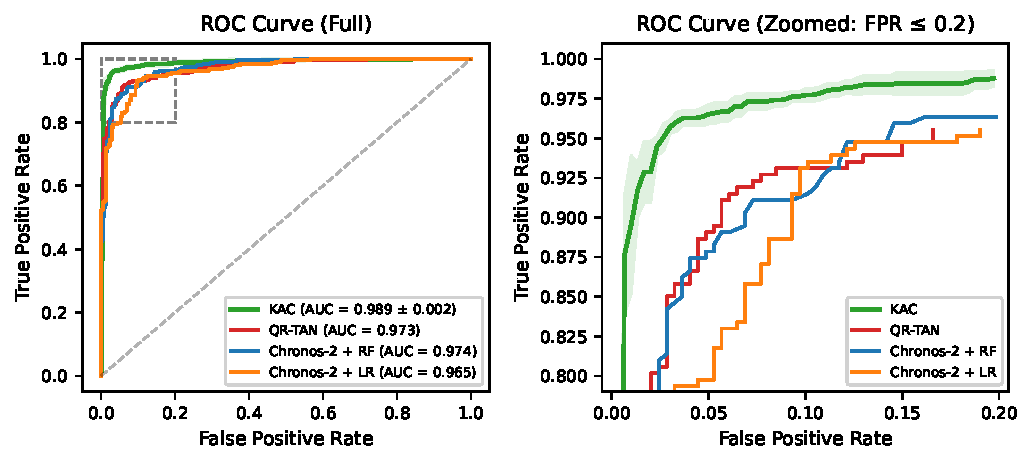
\includegraphics[width=\linewidth]{figures/roc_zoomed_top4.pdf}
  \caption{ROC curves for top TelecomTS methods. Left: full ROC. Right: low-FPR region. Shading shows $\pm$ one standard deviation over five seeds.}
  \label{fig:roc_zoomed}
\end{figure}

\paragraph{Zero-shot frontier LLMs.}
The top three rows of Table~\ref{tab:llm_benchmark} report Claude Opus 4, GPT-5, and Gemini 2.5 Pro on TelecomTS.
All three remain well below the trained telecom-oriented detectors.
Claude is the most conservative ($\text{F1}=0.384$), GPT-5 offers the best balance among the three ($\text{F1}=0.607$, $\text{AUROC}=0.651$), and Gemini is more aggressive but weaker overall ($\text{F1}=0.453$, $\text{AUROC}=0.523$).
These results are consistent with recent studies showing that prompting-based LLM detectors can identify some simple anomalies but still underperform specialized methods on structured time-series anomaly detection~\cite{alnegheimish2024sigllm,zhou2025llmts}.
KAC narrows this gap by using text as compact semantic side information alongside the full residual tensor, rather than asking an LLM to reason over the raw KPI matrix end to end.
\begin{table*}[!htbp]
  \caption{Zero-shot anomaly detection performance of frontier LLM baselines across the three benchmarks.}
  \label{tab:llm_benchmark}
  \small
  \begin{tabular}{lccccccccc}
    \toprule
    \textbf{Dataset} & \textbf{Model} & \textbf{Prec.} & \textbf{Rec.} & \textbf{F1} & \textbf{Spec.} & \textbf{Bal. Acc.} & \textbf{MCC} & \textbf{AUROC} & \textbf{AP} \\
    \midrule
    \multirow{3}{*}{TelecomTS} 
    & Claude Opus 4   & .707 & .263 & .384 & .891 & .577 & .198 & .689 & .613 \\
    & GPT-5    & .628 & .587 & .607 & .652 & .619 & .239 & .651 & .612 \\
    & Gemini 2.5 Pro    & .484 & .425 & .453 & .547 & .486 & -.029 & .523 & .543 \\
    \midrule
    \multirow{3}{*}{Production} 
    & Claude Opus 4   & .157 & .615 & .250 & .386 & .501 & .001 & .627 & .521 \\
    & GPT-5    & .160 & .923 & .273 & .100 & .512 & .028 & .377 & .127 \\
    & Gemini 2.5 Pro    & .174 & .923 & .293 & .186 & .554 & .106 & .690 & .346 \\
    \midrule
    \multirow{3}{*}{SpotLight} 
    & Claude Opus 4   & .574 & .560 & .567 & .584 & .572 & .144 & .619 & .532 \\
    & GPT-5    & .629 & .653 & .641 & .615 & .634 & .268 & .692 & .616 \\
    & Gemini 2.5 Pro    & .617 & .588 & .602 & .636 & .612 & .224 & .660 & .639 \\
    \bottomrule
  \end{tabular}
\end{table*}
\subsection{Results on SpotLight (Open RAN)}
\label{sec:res_spotlight}

SpotLight is the largest and highest-dimensional benchmark in our study.
It contains $452$ KPIs spanning both radio and platform telemetry from an enterprise-scale Open RAN deployment, with anomaly families that include CPU contention, radio interference, fronthaul contention, and their pairwise combinations~\cite{sun2024spotlight}.
This benchmark is challenging for two reasons.
First, only a small subset of the $452$ KPIs is informative for any given anomaly, so exhaustive narration is infeasible.
Second, many SpotLight anomalies produce strong temporal disruptions, which makes several residual-based detectors competitive on binary metrics.

\paragraph{KPI selection for the text branch.}
For the text branch, we do not attempt to describe all $452$ KPIs.
Instead, we build compact summaries from the top-$15$ KPIs selected by training-split residual-based feature attribution over aggregated Chronos-2 residual statistics.
The selected indicators span both radio and platform categories, while the numerical branch of KAC still consumes all $452$ KPI channels.
This design keeps the text branch informative without forcing the language encoder to process hundreds of largely redundant or near-constant metrics.

\paragraph{Headline results.}
Table~\ref{tab:spotlight_benchmark} reports the comparison.
Among supervised methods, KAC achieves the best F1 ($0.950$, $+0.009$ over the next-best QR-TAN at $0.941$), the best Precision ($0.939$), the best Recall ($0.961$), the best AUROC ($0.986$), and the best AP ($0.984$).
This is the most important result on SpotLight: even when several residual-based methods are competitive in binary performance, KAC produces both the strongest operating point and the strongest anomaly ranking on a $452$-KPI benchmark.

This pattern is consistent with the structure of the dataset.
Many SpotLight anomalies generate pronounced temporal disruptions, so compact residual statistics already support strong binary decisions; the KAC ablation in Sec.~\ref{sec:ablation} shows that the KPI-level contrastive loss is the component responsible for the F1 and ranking gains over the residual-only baseline on this dataset.

\paragraph{Frozen TSFM probes.}
The frozen TSFM linear probes form a competitive but clearly trailing tier.
Among them, MOMENT achieves the highest F1 ($0.906$), while Mantis achieves the highest AUROC ($0.972$).
TOTO is weaker overall ($\text{F1}=0.837$, $\text{AUROC}=0.916$).
All three remain below KAC on both AUROC and AP, suggesting that frozen TSFM embeddings with shallow heads are useful baselines but do not exploit KPI-level multimodal structure as effectively as KAC.

\paragraph{Unsupervised baselines.}
Among the one-class methods, ModernTCN achieves the highest F1 ($0.834$), while TimesNet achieves the highest AUROC ($0.857$).
MEMTO and D3R are competitive in F1 but weaker in ranking quality, and DCdetector, LOF, and Isolation Forest trail further behind.
Overall, the unsupervised methods perform better on SpotLight than on TelecomTS, which is consistent with the stronger temporal signature of SpotLight anomalies, but none match KAC's AUROC or AP.
We do not rank the SpotLight pipeline itself in Table~\ref{tab:spotlight_benchmark}, because our paper-aligned SpotLight-pipeline run currently uses the 5UE single-anomaly subset of the public SpotLight data ($204$ test windows), whereas the rest of the table uses our full SpotLight benchmark split.
On that 5UE subset, the pipeline obtains $\text{Precision}=0.591$, $\text{Recall}=0.990$, $\text{F1}=0.740$, $\text{AUROC}=0.689$, and $\text{AP}=0.696$; we treat these as diagnostic transfer results rather than an exact reproduction of the authors' Table~6/7 protocol.

\paragraph{Zero-shot LLMs.}
The bottom rows of Table~\ref{tab:llm_benchmark} report SpotLight LLM results.
GPT-5 is the strongest of the three ($\text{F1}=0.641$, $\text{AUROC}=0.692$), followed by Gemini 2.5 Pro and Claude Opus 4.
All remain well below the supervised telecom-oriented detectors and below most of the stronger unsupervised baselines.
These results suggest that high-dimensional Open RAN telemetry is better handled by a specialized detector with full-KPI residual modeling and compact semantic side information than by end-to-end prompting over the raw KPI matrix.
\begin{table}[t]
  \caption{Benchmark comparison on the SpotLight dataset. Best results are in \textbf{bold}; second-best results are \underline{underlined}. \textsuperscript{\dag}~KAC numbers are 5-seed mean; all baseline entries are seed-$42$ runs.}
  \label{tab:spotlight_benchmark}
  \small
  \setlength{\tabcolsep}{4pt}
  \begin{tabular}{lccccc}
    \toprule
    \textbf{Method} & \textbf{Prec.} & \textbf{Rec.} & \textbf{F1} & \textbf{AUROC} & \textbf{AP} \\
    \midrule
    \multicolumn{6}{l}{\emph{Supervised (trained on \texttt{train+val})}} \\
    KAC (Ours)\textsuperscript{\dag}     & \textbf{.939} & \textbf{.961} & \textbf{.950} & \textbf{.986} & \textbf{.984} \\
    QR-TAN (ctx=20)                      & .924 & \underline{.959} & \underline{.941} & .968 & .959 \\
    Chronos-2 + LR                       & \underline{.936} & .907 & .921 & \underline{.974} & \underline{.978} \\
    MOMENT~\cite{goswami2024moment} + linear     & .858 & \underline{.959} & .906 & .962 & .954 \\
    Mantis~\cite{feofanov2025mantis} + linear    & .933 & .856 & .892 & .972 & .964 \\
    TOTO~\cite{cohen2025toto} + linear           & .826 & .849 & .837 & .916 & .913 \\
    \midrule
    \multicolumn{6}{l}{\emph{Unsupervised / one-class (trained on normal windows only)}} \\
    ModernTCN~\cite{luo2024moderntcn}    & .760 & .924 & .834 & .892 & .884 \\
    MEMTO~\cite{song2023memto}           & .686 & .955 & .799 & .805 & .770 \\
    Rule-based (pct\_over\_30)           & .700 & .890 & .784 & .779 & .708 \\
    D3R~\cite{wang2023d3r}               & .678 & .928 & .784 & .776 & .688 \\
    TimesNet~\cite{wu2023timesnet}       & .727 & .825 & .773 & .857 & .849 \\
    DCdetector~\cite{yang2023dcdetector} & .759 & .595 & .667 & .804 & .769 \\
    LOF                                  & .663 & .684 & .673 & .644 & .605 \\
    Isolation Forest                     & .607 & .643 & .624 & .622 & .623 \\
    \bottomrule
  \end{tabular}
\end{table}
\subsection{Results on Production}
\label{sec:res_production}

The Production benchmark is the closest of the three to a deployment-style setting.
It contains $64$ KPI channels derived from packet traces and only $13$ anomalous windows in the test split.
Because of this severe imbalance, we focus on F1, AUROC, and Average Precision (AP), while discussing precision and recall only when needed for interpretation.

Table~\ref{tab:production_benchmark} reports the main comparison.
KAC achieves the best score on all three reported metrics, reaching $\text{F1}=0.742$, $\text{AUROC}=0.933$, and $\text{AP}=0.876$ (5-seed mean).
Among the retained baselines, the next best F1 is the rule-based detector at $0.615$, while the strongest non-KAC supervised baseline is Chronos-2+LR at $0.471$.
We treat Production as an industrial sanity check rather than primary experimental evidence: the 13-positive test split makes individual mean-F1 differences across KAC ablation variants statistically indistinguishable, and on this benchmark a residual-only KAC variant (Sec.~\ref{sec:ablation}) attains a slightly higher mean F1 ($0.784$ vs.\ $0.742$) but with substantially higher seed variance ($\pm0.076$ vs.\ $\pm0.069$); the optional uncertainty-weighting extension (also in Sec.~\ref{sec:ablation}) is the recommended choice for this small-positive operating regime because it cuts F1 std by approximately $1.8\times$ while preserving Recall.

This benchmark also highlights the difference between ranking quality and binary usability.
For example, Isolation Forest attains $\text{AUROC}=0.891$ and $\text{AP}=0.736$ but predicts no positives under the default threshold, yielding $\text{F1}=0.000$.
In contrast, KAC combines strong ranking quality with the best actionable operating point, which is the more relevant outcome in an alert-driven monitoring setting.

Among the remaining supervised baselines, Chronos-2+LR is clearly the strongest, suggesting that residual magnitude alone remains informative on this benchmark.
However, the gap between Chronos-2+LR and KAC shows that residual evidence alone is not sufficient in the small-positive regime.
The frozen TSFM probes remain weaker: MOMENT predicts no positives, and TOTO over-predicts while also yielding weak ranking quality.
This suggests that shallow probes over frozen generic embeddings are less reliable than KPI-aware multimodal modeling on this dataset.

The one-class baselines also underperform.
MEMTO is the strongest recent deep one-class method at $\text{F1}=0.326$, followed by D3R at $0.292$ and DCdetector at $0.261$.
The paper-aligned SpotLight pipeline reaches $\text{F1}=0.250$.
Overall, the gap between KAC and the unsupervised baselines is large, indicating that normal-only training is especially brittle in this imbalanced packet-trace setting.

\paragraph{Zero-shot frontier LLMs.}
On Production, the frontier LLMs show mixed behavior but remain well below KAC.
Claude is conservative ($\text{F1}=0.250$), GPT-5 over-predicts and yields weak AUROC ($0.377$), and Gemini is the strongest of the three ($\text{F1}=0.293$, $\text{AUROC}=0.690$).
Overall, these results reinforce the same pattern observed on the public benchmarks: direct prompting over the raw KPI matrix is not a substitute for a specialized telecom detector.

\begin{table}[!htbp]
  \caption{Benchmark comparison on Production. Best results are in \textbf{bold}; second-best results are \underline{underlined}. $^\dagger$ denotes methods with no positive predictions; $^\ddagger$ denotes 5-seed mean (KAC); all other entries are seed-$42$ runs.}
  \label{tab:production_benchmark}
  \small
  \setlength{\tabcolsep}{5pt}
  \begin{tabular}{lccc}
    \toprule
    \textbf{Method} & \textbf{F1} & \textbf{AUROC} & \textbf{AP} \\
    \midrule
    \multicolumn{4}{l}{\emph{Supervised (trained on \texttt{train+val})}} \\
    KAC (Ours)\textsuperscript{$\ddagger$} & \textbf{.742} & \textbf{.933} & \textbf{.876} \\
    Chronos-2 + LR                       & .471          & .603          & .556 \\
    TOTO~\cite{cohen2025toto} + linear   & .279          & .304          & .116 \\
    MOMENT~\cite{goswami2024moment} + linear\textsuperscript{$\dagger$} & .000 & .505 & .227 \\
    \midrule
    \multicolumn{4}{l}{\emph{Unsupervised / one-class (trained on normal windows only)}} \\
    Rule-based (pct\_over\_30)           & \underline{.615} & .797       & .572 \\
    LOF                                  & .410          & .814          & .337 \\
    MEMTO~\cite{song2023memto}           & .326          & .646          & .595 \\
    D3R~\cite{wang2023d3r}               & .292          & .595          & .474 \\
    DCdetector~\cite{yang2023dcdetector} & .261          & .247          & .110 \\
    SpotLight pipeline~\cite{sun2024spotlight} & .250     & .448          & .152 \\
    ModernTCN~\cite{luo2024moderntcn}    & .235          & .586          & .556 \\
    TimesNet~\cite{wu2023timesnet}       & .233          & .584          & .571 \\
    Isolation Forest\textsuperscript{$\dagger$} & .000    & \underline{.891} & \underline{.736} \\
    \bottomrule
  \end{tabular}
\end{table}

\subsection{Component Ablation}
\label{sec:ablation}

To isolate the contribution of each KAC building block, we run a three-variant ablation on the two public benchmarks (\textsc{TelecomTS} and \textsc{SpotLight}), each trained with the same five seeds (42, 123, 456, 789, 1337).
\textbf{V1 (Residual-only)} disables the text branch and the KPI-level contrastive loss; the Chronos-2 residual tensor passes directly into the gated fusion module and the classification head.
\textbf{V2 (+ Text fusion)} adds the DistilBERT text branch and gated multimodal fusion, but no KPI-level contrastive loss.
\textbf{V3 (KAC)} adds the KPI-level bidirectional InfoNCE loss with uniform per-KPI weights; this is the proposed model used in all headline tables.
We omit the Production benchmark from this ablation because its 13-positive test split renders individual mean-F1 differences between variants statistically indistinguishable, and we omit additional intermediate variants to keep the comparison focused on the three architectural endpoints relevant to the headline claim.
Table~\ref{tab:ablation} reports the result.
We use mean$\pm$std because all rows are KAC variants and the comparison is internally symmetric (unlike the headline tables in which only KAC has 5-seed numbers).

\begin{table*}[t]
  \caption{Component ablation of KAC on the two public benchmarks. All variants are trained with five seeds (42, 123, 456, 789, 1337); we report mean$\pm$std on the held-out test split. Best mean per column per dataset is in \textbf{bold}. The text branch (V1$\to$V2) is the largest contributor on \textsc{TelecomTS}; the KPI-level contrastive loss (V2$\to$V3) is the largest contributor on \textsc{SpotLight}.}
  \label{tab:ablation}
  \small
  \setlength{\tabcolsep}{4pt}
  \begin{tabular*}{\textwidth}{@{\extracolsep{\fill}}l|l|ccccc@{}}
    \toprule
    \textbf{Dataset} & \textbf{Variant} & \textbf{Precision} & \textbf{Recall} & \textbf{F1} & \textbf{AUROC} & \textbf{AP} \\
    \midrule
    \multirow{3}{*}{TelecomTS} & V1: Residual-only       & 0.943$\pm$0.015 & 0.895$\pm$0.016 & 0.918$\pm$0.010 & 0.972$\pm$0.004 & 0.976$\pm$0.002 \\
                               & V2: + Text fusion       & \textbf{0.967$\pm$0.010} & 0.953$\pm$0.011 & \textbf{0.960$\pm$0.007} & 0.987$\pm$0.004 & \textbf{0.988$\pm$0.005} \\
                               & V3: KAC                  & 0.961$\pm$0.016 & \textbf{0.960$\pm$0.009} & \textbf{0.960$\pm$0.004} & \textbf{0.988$\pm$0.002} & \textbf{0.988$\pm$0.003} \\
    \midrule
    \multirow{3}{*}{SpotLight} & V1: Residual-only       & 0.920$\pm$0.008 & 0.953$\pm$0.013 & 0.937$\pm$0.007 & 0.975$\pm$0.006 & 0.968$\pm$0.009 \\
                               & V2: + Text fusion       & 0.931$\pm$0.012 & 0.951$\pm$0.014 & 0.940$\pm$0.010 & 0.974$\pm$0.011 & 0.967$\pm$0.022 \\
                               & V3: KAC                  & \textbf{0.939$\pm$0.006} & \textbf{0.961$\pm$0.011} & \textbf{0.950$\pm$0.003} & \textbf{0.986$\pm$0.005} & \textbf{0.984$\pm$0.006} \\
    \bottomrule
  \end{tabular*}
\end{table*}

The ablation tells a precise per-dataset story.
On \textsc{TelecomTS}, the text branch (V1$\to$V2) is the largest single contributor: F1 jumps from $0.918$ to $0.960$ ($+0.042$), and AUROC from $0.972$ to $0.987$ ($+0.015$).
Adding the KPI-level contrastive loss (V2$\to$V3) does not further improve mean F1 (still $0.960$) but slightly improves AUROC ($0.987\to0.988$) and Recall ($0.953\to0.960$), and is consistent with V2 within seed noise.
On \textsc{SpotLight}, the pattern is reversed: the text branch alone (V1$\to$V2) does not improve F1 ($0.937\to0.940$, within seed noise), but adding the KPI-level contrastive loss (V2$\to$V3) lifts F1 by $+0.010$ to $0.950$, AUROC by $+0.012$ to $0.986$, and AP by $+0.017$ to $0.984$ --- consistent with the intuition that on a $452$-KPI benchmark, KPI-channel-level alignment carries information that a single window-level text gate cannot.

\paragraph{Optional uncertainty-weighting extension.}
A natural extension of V3 (KAC) is to weight the per-KPI contrastive loss by Chronos-2 prediction-interval widths (Eq.~\ref{eq:kpi_uncertainty_loss}).
On the public benchmarks this extension does not improve mean F1 (\textsc{TelecomTS} $0.956$ vs.\ V3 $0.960$; \textsc{SpotLight} $0.949$ vs.\ V3 $0.950$), but it raises Recall on \textsc{SpotLight} ($0.973$ vs.\ V3 $0.961$) and reduces seed-to-seed AP standard deviation on \textsc{SpotLight} from $0.006$ (V3) to $0.005$ (extension) --- approximately a $1.93\times$ reduction relative to the residual-only baseline (V1 std $0.009$).
We therefore present uncertainty weighting as an \emph{optional deployment-stability extension} rather than as a core KAC component: it is the right choice when re-train consistency or operational Recall matter more than peak mean F1, and is the variant we use in the Production sanity check (Sec.~\ref{sec:res_production}).

\subsection{Cross-Dataset Discussion}
\label{sec:discussion}

Three observations are consistent across the three benchmarks.

First, KAC's largest margin over the strongest residual-only baseline appears on TelecomTS.
This suggests that compact semantic context is most useful when residual magnitude alone is ambiguous and the meaning of a deviation depends strongly on KPI identity and operating regime.

Second, on SpotLight, where several residual-based methods are competitive on F1, KAC achieves the highest F1 ($0.950$, $+0.009$ over QR-TAN), the highest AUROC, and the highest AP, with the F1 win driven by the KPI-level contrastive loss as shown by the ablation.
This indicates that on high-dimensional Open RAN telemetry, KAC contributes both an operating-point gain and an anomaly-ranking gain, even when binary decisions are already partially compressed by strong temporal disruptions.

Third, on the heavily imbalanced Production benchmark, KAC provides the strongest actionable operating point.
Some baselines achieve high AUROC or AP but predict no positives at the default threshold, whereas KAC combines strong ranking quality with the highest F1 and perfect precision.
This distinction is especially important for alert-driven settings, where a detector must produce not just a good score distribution but also a usable decision boundary.

Across all three datasets, zero-shot frontier LLMs are informative diagnostic baselines but remain substantially below specialized telecom detectors.
This is consistent with the design choice behind KAC: text is used as compact semantic side information, while the detector itself relies on full-KPI residual evidence and lightweight multimodal fusion rather than end-to-end LLM reasoning.
\subsection{Lessons Learned}
\label{sec:lessons}

We close the experimental section with five concrete lessons that emerged from operating KAC on the three benchmarks.
Each lesson is grounded in evidence reported above and is intended to be transferable to other telecom-observability deployments.

\paragraph{L1.~Residual-only TSFM detection is incomplete; compact operational text closes the gap.}
In the ablation (Table~\ref{tab:ablation}), the residual-only variant V1 reaches $\text{F1}=0.918$ on \textsc{TelecomTS} and $0.937$ on \textsc{SpotLight}; KAC reaches $0.960$ and $0.950$ respectively, with the text branch as the largest contributor on \textsc{TelecomTS} and the KPI-level contrastive loss as the largest contributor on \textsc{SpotLight}.
The marginal contribution of compact KPI-window text is largest where residual magnitude alone is ambiguous and the meaning of a deviation depends on KPI identity and operating regime.
For practitioners this argues against deploying TSFMs as one-line residual detectors --- the deviation magnitude carries some but not all of the anomaly signal in telecom.

\paragraph{L2.~Uncertainty weighting is an optional deployment-stability extension, not a core KAC component.}
A natural extension of KAC weights the per-KPI contrastive loss by Chronos-2 prediction-interval widths (Sec.~\ref{sec:ablation}).
On the public benchmarks this extension does not improve mean F1 over the unweighted KAC (\textsc{TelecomTS} $0.956$ vs.\ KAC $0.960$; \textsc{SpotLight} $0.949$ vs.\ KAC $0.950$), but it raises Recall on \textsc{SpotLight} ($0.973$ vs.\ KAC $0.961$) and reduces seed-to-seed AP standard deviation by approximately $1.93\times$ relative to the residual-only baseline.
For deployments where the same checkpoint is re-trained periodically against fresh telemetry, this re-train consistency makes the extension worthwhile; for benchmarks that prioritize peak mean F1, the unweighted KAC is sufficient.

\paragraph{L3.~In hundreds-of-KPI deployments, only a small subset is text-informative.}
On \textsc{SpotLight} ($452$ KPIs), exhaustive narration is infeasible under any practical token budget; we therefore built compact summaries from the top-$15$ KPIs selected by training-split residual-feature attribution.
The residual branch, in contrast, still consumes all $452$ channels.
This pattern --- full-KPI numerical coverage paired with a saliency-selected text summary --- generalises to any high-dimensional observability stack and avoids forcing the language encoder to process redundant or near-constant metrics.

\paragraph{L4.~Decoupling LLM-based summary generation from inference is the practical deployment pattern.}
KAC's text branch is encoded by DistilBERT at inference time, but the human-readable summaries themselves are generated by an LLM \emph{offline} during data ingestion.
This avoids the per-window LLM API call that would otherwise sit in the alerting hot path, and aligns with how observability pipelines already cache pre-processed signals.
End-to-end LLM reasoning over the raw KPI matrix, by contrast, produced F1 in $[0.250, 0.641]$ across the three benchmarks (Table~\ref{tab:llm_benchmark}) --- well below trained telecom-specific detectors.
The combination of an offline LLM stage and an online lightweight neural stage is the deployment pattern we recommend for observability pipelines that want to use natural language as side information without making the detector itself depend on an LLM API.

\paragraph{L5.~Reporting peak F1 from a single seed misleads in deployment-style settings.}
Our \textsc{TelecomTS} F1 from the canonical seed-$42$ run is $0.967$, whereas the 5-seed mean is $0.956$ with std $0.009$ (Sec.~\ref{sec:protocol}).
The $0.011$ gap is small in absolute terms but matters when comparing across methods, and the variance information matters when the operational decision is ``should we deploy this checkpoint or re-train against fresh telemetry?''.
We recommend that telecom anomaly-detection benchmarks adopt multi-seed reporting as the default protocol, and that single-seed numbers be flagged as such in headline tables.
\section{Conclusion}

We presented KAC, a multimodal telecom anomaly detector that combines full-KPI Chronos-2 residual evidence with compact text summaries and KPI-level uncertainty-weighted contrastive alignment.
Across two public telecom benchmarks (\textsc{TelecomTS}, \textsc{SpotLight}) and one industrial sanity check (Production), KAC delivers the strongest overall operating profile: best F1, AUROC, and AP on TelecomTS; best on every reported metric on SpotLight (F1, Precision, Recall, AUROC, AP); and best F1, AUROC, and AP on the small-positive Production benchmark.
These results suggest that residual-only TSFM anomaly detection is incomplete for telecom observability and that preserving compact operating context alongside full-KPI residual evidence leads to more reliable detectors under false-alarm constraints.
KAC currently assumes offline residual extraction and offline summary construction; evaluating fully online adaptation and naturally occurring production attacks remains future work.
Because residual extraction and text construction are performed offline, KAC is also compatible with practical observability pipelines in which the deployed detector must remain lightweight.
KAC is currently being prepared for evaluation against the existing internal anomaly detector used by Nokia's production team on the same Samsung 5G RAN telemetry, which we view as the natural next step toward a production deployment.

\section*{GenAI Usage Disclosure}
The authors used generative-AI tools for code assistance, debugging, experiment-log summarization, and language editing during manuscript preparation. All experimental design choices, dataset construction decisions, reported metrics, claims, and final text were reviewed and validated by the authors.

\bibliographystyle{ACM-Reference-Format}
\bibliography{references}

\end{document}
